% Schritt 6: Auswertung
% - Effekte ermitteln, Signifikanz prüfen (Modellreduzierung!), R2-Werte; dabei
% Datenqualität prüfen (z. B. echte Ausreißer dürfen nicht ausgewertet werden!
% Einzelversuche wiederholen, neue Reduzierung)
% - Überprüfung der Modellvoraussetzungen nach jeder Modellreduzierung
% - Regressionsgleichung aufstellen, graphische Darstellung
\chapter{Ergebnisse}\label{ch:ergebnisse}

% 1. Analyse des vollständigen Modells und erste Diagnostik der Residuen
% Anhand der Varianzanalyse der Effekte wird abgeschätzt, welche Faktoren aufgrund des geringen Effekts kaum signifikant
% resp. für die Praxis nicht relevant sind. Eine erste graphische Residuendiagnostik wird durchgeführt, um grobe Abweichungen
% früh erkennen zu können.
\paragraph{Die Analyse des vollständigen Modells} zeigt das Modell ist klar signifikant ($p \le 0,001$).
Der R²-Wert (98,35\,\%) und der korrigierte R²-Wert (97,49\,\%) liegen nahe beieinander und nahe 100\,\%.
Das spricht für ein gutes Modell. % (siehe Abbildung \ref{fig:modell_gesamt}).
Alle drei Haupteffekte sind klar signifikant ($p \le 0,001$).
Die Zuckermenge wirkt sich am stärksten und positiv auf den Durchmesser aus ($13,542$),
gefolgt vom Anteil an Vollkornmehl ($-9,292$) mit einen negativen Effekt.
Die Buttermenge erzielt ebenfalls eine positiv Effekt ($8,292$) auf den Durchmesser.
Bei den Wechselwirkungen sind nur \emph{Butter*Zucker} und \emph{Zucker*Vollkornmehl} signifikant ($p \le 0,05$).
Die 2FWW \emph{Butter*Zucker} erreicht einen p-Wert von $0,032$ und hat mit $1,292$ nur einen geringen Effekt im Vergleich zu den Haupteffekten.
\emph{Zucker*Vollkornmehl} wirkt sich im gleichen Maß negativ auf den Durchmesser aus ($-1,292$) mit dem gleichen p-Wert wie \emph{Butter*Zucker}.

Die Krümmung zeigt Signifikanz ($p \le 0,05$) mit einem p-Wert von $0,033$.
Der Zentralpunkt ist mit den gleichem p-Wert signifikant.
Das deutet darauf hin, dass mindestens ein Faktor im Modell einen nicht-linearen Einfluss hat.
Der experimentelle Zentralpunkt liegt $1,438$ Einheiten unter dem errechneten Zentralpunkt ($71,771$) des Modells.
Bei den Blöcken zeigt Block 1 klare Signifikanz ($p \le 0,001$), während Block 2 mit einem p-Wert von $0,744$ nicht signifikant ist.
Die Blockbildung im Gesamten erreicht aber einen p-Wert von $0,000$.
Die Abbildung \ref{fig:analyse_gesamt} zeigt die relevanten Diagramme der Analyse.
Die Ergebnisse dazu sind im Anhang \ref{ch:appendix_ergebnisse} zu finden.

Die Regressionsgleichung für das vollständige Modell mit kodierten Einheiten ist wie folgt:

\begin{equation} \label{eq:modell_gesamt}
\begin{split}
\text{Durchsch\_Durchmesser} = & 71,771 - 1,583 \cdot \text{Block\_1} + 0,117 \cdot \text{Block\_2}  \\
    & + 4,146 \cdot \text{Butter} + 6,771 \cdot \text{Zucker} - 4,646 \cdot \text{Vollkornmehl} \  \\
    & + 0,646 \cdot (\text{Butter}\cdot\text{Zucker}) - 0,521 \cdot (\text{Butter}\cdot\text{Vollkornmehl})  \\
    & - 0,646 \cdot (\text{Zucker}\cdot\text{Vollkornmehl}) \\
    & + 0,312 \cdot (\text{Butter}\cdot\text{Zucker}\cdot\text{Vollkornmehl})  \\
    & - 1,438 \cdot \text{ZtrPkt}
\end{split}
\end{equation}

\begin{figure}
    \centering
\begin{subfigure}{0.49\textwidth}
    \centering
    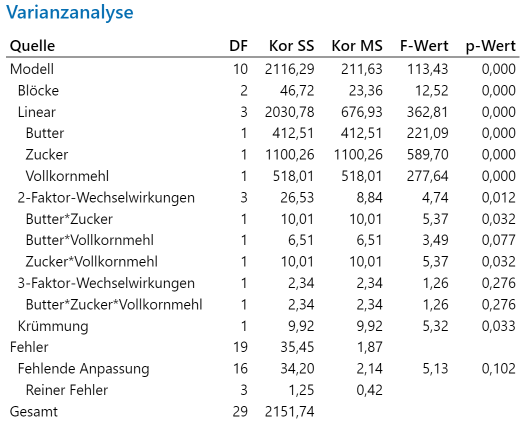
\includegraphics[width = \textwidth]{figures/varianzanalyse_gesamt.png}
    \caption{Varianzanalyse des vollständigen Modells}
    \label{fig:anova_gesamt}
\end{subfigure}\hfill
\begin{subfigure}{0.49\textwidth}
    \centering
    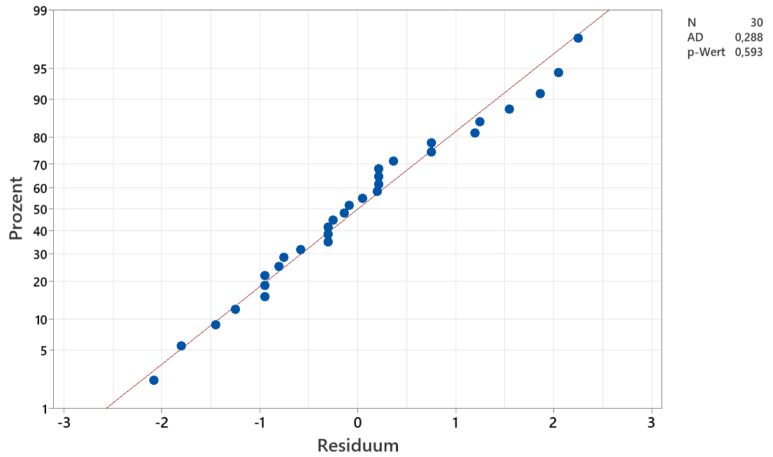
\includegraphics[width = \textwidth]{figures/wahrscheinlichkeitsnetz_gesamt.png}
    \caption{Wahrscheinlichkeitsnetz für die Normalverteilung}
    \label{fig:wahrscheinlichkeitsnetz_gesamt}
\end{subfigure}

\medskip

\begin{subfigure}{0.49\textwidth}
    \centering
    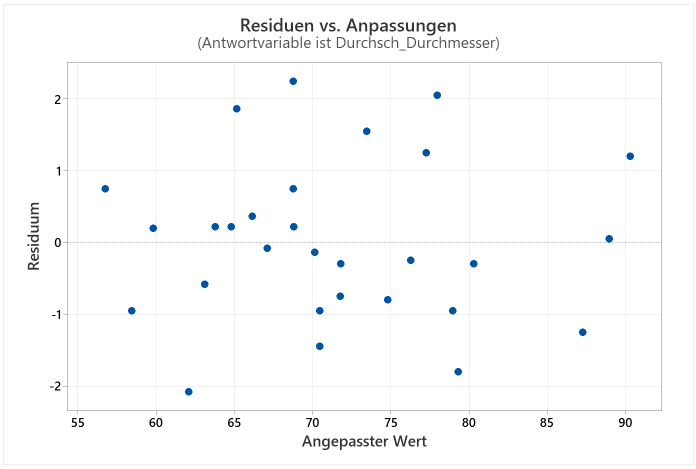
\includegraphics[width = \textwidth]{figures/residuen_anpassung_gesamt.png}
    \caption{Residuen in Abhängigkeit der Prognosewerte}
    \label{fig:residuen_anpassung_gesamt}
\end{subfigure}\hfill
\begin{subfigure}{0.49\textwidth}
    \centering
    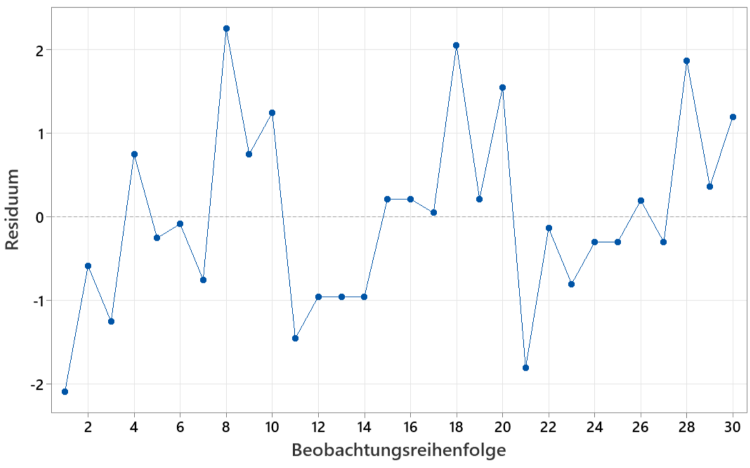
\includegraphics[width = \textwidth]{figures/residuen_reihenfolge_gesamt.png}
    \caption{Residuen in Abhängigkeit der Durchläufe}
    \label{fig:residuen_reihenfolge_gesamt}
\end{subfigure}

\caption{Analyse des vollständigen Modells}
\label{fig:analyse_gesamt}

\end{figure}

Die graphische Analyse der Residuen gibt keinen Hinweis auf eine Abweichungen der Normalverteilung (siehe Abbildung \ref{fig:wahrscheinlichkeitsnetz_gesamt}).
Zudem zeigt Abbildung \ref{fig:residuen_anpassung_gesamt}, dass die Residuen zufällig um die berechneten Prognosewerte gestreut sind.
Allerdings zeigt sich in der Analyse der Durchlaufnummern ein klar steigender Trend der Residuen innerhalb der Blöcke.
Die Blöcke haben die Durchlaufnummern 1-10, 11-20 und 21-30.
Dieser Trend ist auf die Blechposition zurück zu führen.
Die Positionen 1, 2 und 3 liegen hinten im Ofen während die Positionen 8, 9 und 10 vorne liegen.
Die Werte der Durchlaufnummer 1, 8, und 18 liegen dabei in einem kritischen Bereich.
Um diesen Trend auszugleichen wurden die Positionen randomisiert und strukturiert rotiert.
%Deshalb wird als nächstes mit der Modellreduzierung fortgefahren.

% 2. Vereinfachung des Modells
% Entfernen Sie nach und nach alle nicht signifikanten Terme aus dem Modell. Gehen Sie dabei sukzessive vor und entfernen
% Sie schrittweise immer den Effekt mit dem höchsten p-Wert, solange bis alle Effekte signifikant sind (Anmerkungen zur
% Hierarchie beachten). Zuerst Blöcke und Zentralpunkte entfernen (sofern nicht signifikant), dann weitere Terme.
\paragraph{Die Modellvereinfachung} beginnt mit der 3FWW \emph{Butter*Zucker*Vollkornmehl}, weil diese mit $0,276$ den größten p-Wert aufweist.
Zentralpunkt und die Blockbildung bleibt aufgrund der Signifikanz vorerst erhalten.
Durch die Vereinfachung weichen die Prognosen für die Durchlaufnummern 1 und 18 stärker ab.
Diese werden von MiniTab als \emph{ungewöhnliche Beobachtung} ausgewiesen und bewertet (siehe Abbildung \ref{fig:vereinfachung_1}).
Diese Beobachtungen sind auf die Blechpositionen zurückzuführen.
Der Fehler des Modells bleibt bei der \emph{Fehlenden Anpassung} allerdings nicht signifikant.
Auch die Residuen weichen nicht stark vom vorherigen Modell ab.

\begin{figure}
    \centering
    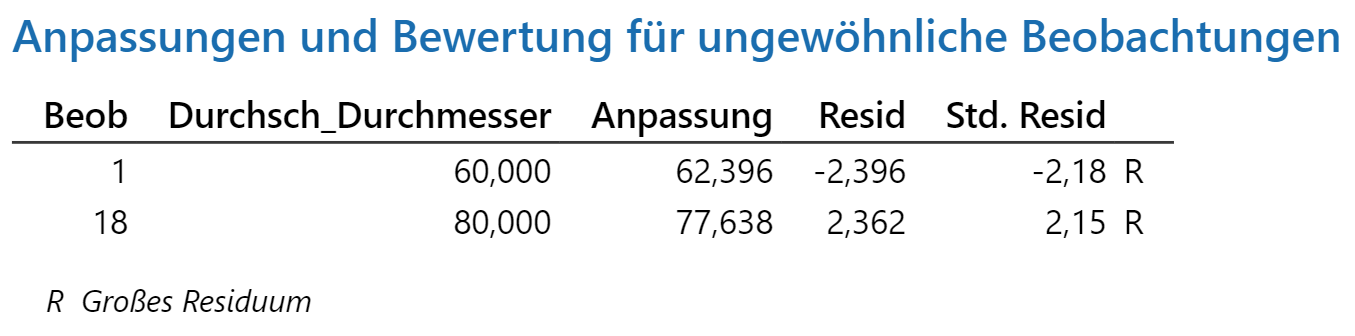
\includegraphics[width=\linewidth]{figures/anpassungen_vereinfachung_1.png}
    \caption{Ungewöhnliche Beobachtungen nach der ersten Vereinfachung}
    \label{fig:vereinfachung_1}
\end{figure}

Als nächstes wird die 2FWW \emph{Butter*Vollkornmehl} entfernt.
Diese weißt mit einem p-Wert von $0,078$ als nächste Wechselwirkungen keine Signifikanz auf.
Durch die Vereinfachung wird nur noch die Prognose für die Durchlaufnummern 1 als \emph{ungewöhnliche Beobachtung} ausgewiesen.
Die Residuen-Analyse ergibt keine Hinweise auf Änderungen in der Normalverteilung, Streuung oder in der Ablaufstruktur.
Damit sind für $p < 0,05$ alle nicht Signifikaten Faktoren und Wechselwirkungen entfernt.
Allerdings bleibt noch immer der Hinweis auf eine Krümmung mit dem p-Wert von $0,042$.

Darum wird für die weitere Vereinfachung das Signifikanzniveau von 5\,\% auf 1\,\% angehoben.
Damit wird als nächstes der Zentralpunkt aufgrund von fehlender Signifikanz aus dem Modell entfernt.
Für das neue Modell ergeben sich noch immer gute Werte für  R² (97,48\,\%) und R²(kor.) (96,68\,\%).
Allerdings wird ein Durchlauf mehr (1 und 20) als \emph{ungewöhnliche Beobachtung} ausgewiesen (siehe Abbildung \ref{fig:vereinfachung_3})
Die \emph{Fehlenden Anpassung} ist weiterhin nicht signifikant, genau wie nun auch die 2FWW \emph{Butter*Zucker} und \emph{Zucker*Vollkornmehl}.
Die Residuen zeigen weiterhin Normalverteilung mit zufälliger Streuung, und den Trend der Blechpositionen.

\begin{figure}
    \centering
    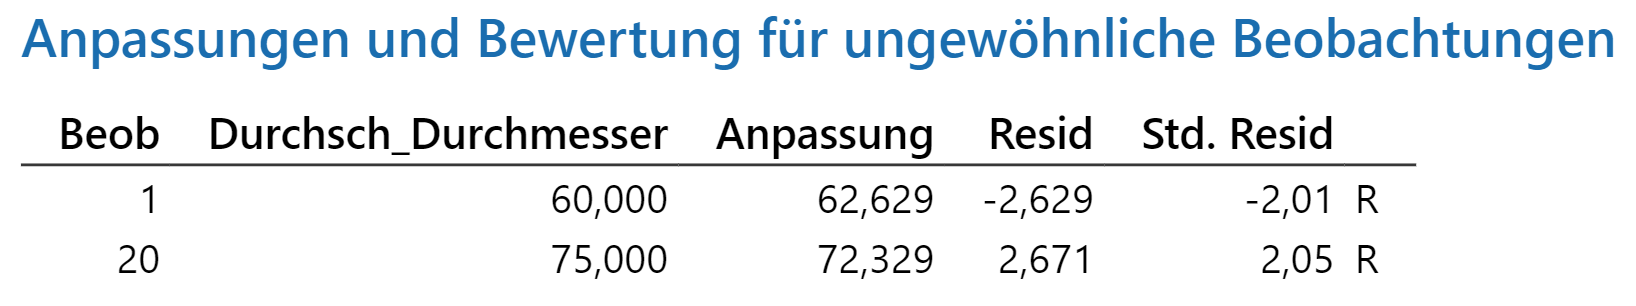
\includegraphics[width=\linewidth]{figures/anpassungen_vereinfachung_3.png}
    \caption{Ungewöhnliche Beobachtungen nach der dritten Vereinfachung}
    \label{fig:vereinfachung_3}
\end{figure}

Im nächsten Schritt wird die 2FWW \emph{Butter*Zucker} entfernt.
Dabei ergeben kaum Änderungen.
Nur der Durchlauf mit der Nummer 20 wird nichtmehr als \emph{ungewöhnliche Beobachtung} ausgewiesen.
Zudem steigt der p-Wert für die 2FWW \emph{Zucker*Vollkornmehl} auf $0,071$.
Diese Wechselwirkung wird im nächsten Schritt entfernt.
Das resultierende Modell aus der Vereinfachung ist final.

% 3. Diagnostik (des endgültigen Modells)
% Rechnen Sie das endgültige Modell erneut und führen Sie die dann finale Modelldiagnose durch. Prüfen Sie, ob die Residuen
% normalverteilt sind, ob sie zeitlich konstant sind und ob die Varianz der Residuen konstant ist. Prüfen Sie zudem den R2-Wert
% sowie den korrigierten R2-Wert (Zielwert > etwa 70 %)!
% Werfen Sie einen Blick auf den Lack of Fit und auf ungewöhnliche Beobachtungen (müssen ggf. einzelne Versuche neu
% durchgeführt werden, falls sich ein Ausreißer bestätigt)!
\paragraph{Das finale Modell} beinhaltet nur noch die drei Haupteffekt.
Diese sind alle klar signifikant.
Auch die Blockbildung ist weiterhin sehr signifikant mit einem p-Wert von $0,003$.
Der Block 1 hat einen p-Wert von $0,002$ während der Block 2 mit $0,799$ nichtmehr signifikant ist.
Der R²-Wert (96,55\,\%) und der korrigierte R²-Wert (95,83\,\%) liegen nahe beieinander und nahe 100\,\%.
Damit hat die Modellleistung zwar etwas abgenommen, ist aber mit sehr signifikanten Faktoren noch immer sehr gut.
Der Hinweis auf Krümmung ist nicht signifikant.
Es wird von Linearität ausgegangen.
Der p-Wert für die \emph{Fehlenden Anpassung} liegt bei $0,060$ und weist auf keine Signifikanz.
Dass der Wert sehr niedrig ist, kann unter anderem an den Ausreißern liegen.
Der Durchlauf mit der Nummer 9 wird nun als \emph{ungewöhnliche Beobachtung} ausgewiesen.
Bei Analyse der Residuen zeigt sich, dass es keine Hinweis gegen eine Normalverteilung gibt (siehe Abbildung \ref{fig:wahrscheinlichkeitsnetz_final}).
Die Residuen streuen relativ stark, sind aber zufällig um die Prognosewerte verteilt.
Der Trend der Blechpositionen ist noch erkennbar, nahm aber mit der Vereinfachung des Modells ab.

\begin{figure}
    \centering
\begin{subfigure}{0.47\textwidth}
    \centering
    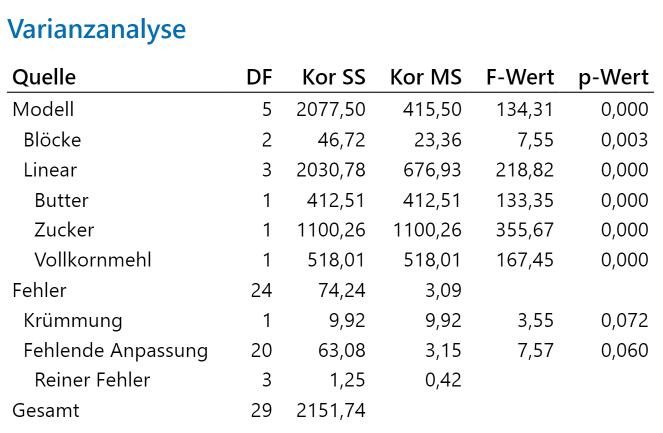
\includegraphics[width = \textwidth]{figures/varianzanalyse_final.png}
    \caption{Varianzanalyse des finalen Modells}
    \label{fig:anova_final}
\end{subfigure}\hfill
\begin{subfigure}{0.47\textwidth}
    \centering
    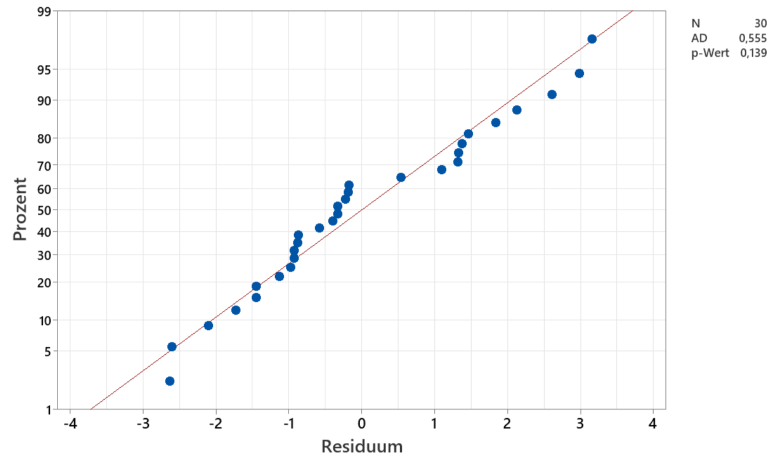
\includegraphics[width = \textwidth]{figures/wahrscheinlichkeitsnetz_final.png}
    \caption{Wahrscheinlichkeitsnetz für die Normalverteilung}
    \label{fig:wahrscheinlichkeitsnetz_final}
\end{subfigure}

\medskip

\begin{subfigure}{0.47\textwidth}
    \centering
    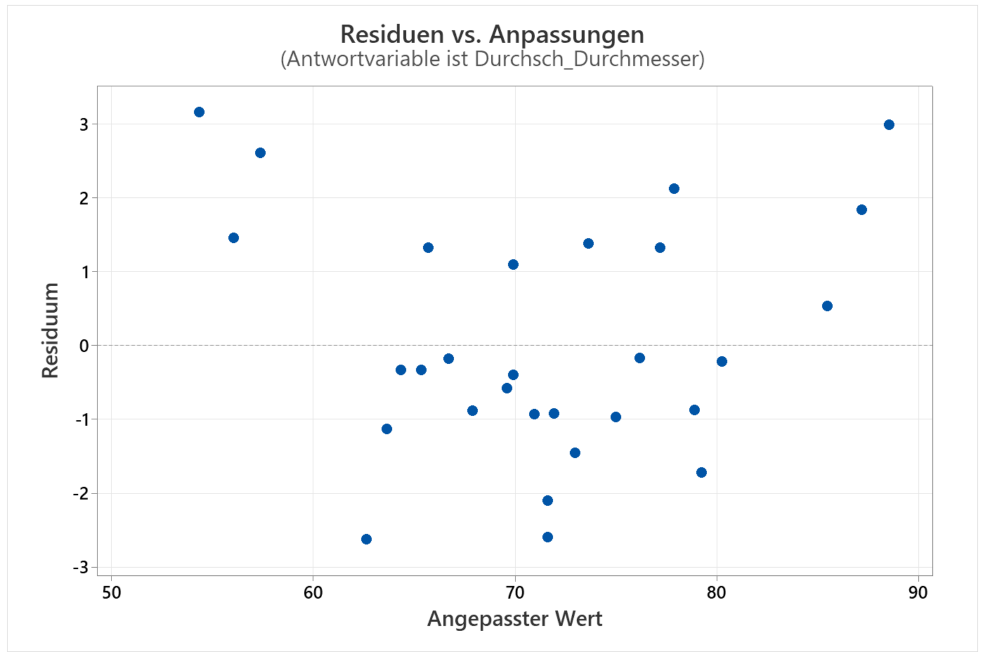
\includegraphics[width = \textwidth]{figures/residuen_anpassung_final.png}
    \caption{Residuen in Abhängigkeit der Prognosewerte}
    \label{fig:residuen_anpassung_final}
\end{subfigure}\hfill
\begin{subfigure}{0.47\textwidth}
    \centering
    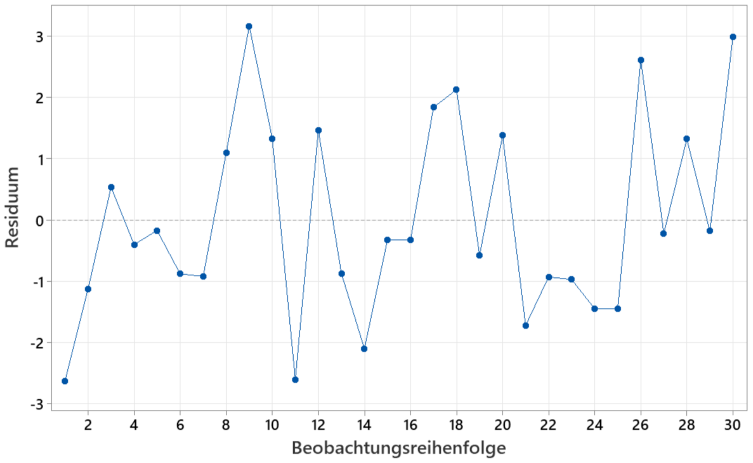
\includegraphics[width = \textwidth]{figures/residuen_reihenfolge_final.png}
    \caption{Residuen in Abhängigkeit der Durchläufe}
    \label{fig:residuen_reihenfolge_final}
\end{subfigure}

\caption{Analyse des finale Modells}
\label{fig:analyse_final}
\end{figure}

% NICHT MÖGLICH
% 4. Ermittlung der optimalen Einstellungen
% Erstellen Sie Wechselwirkungs- und Haupteffekt-Plots bzw. erstellen Sie Cube-Plots. Untersuchen Sie, wo Sie die optimale
% Einstellung finden und ob robuste Prozesseinstellungen vorhanden sind.
% Achtung: Nicht signifikante Effekte sind dabei – trotz graphischer Darstellbarkeit – nicht zu berücksichtigen.
Die Haupteffekt erzielen die gleichen Effekte wie im vollständigen Modell.
Mehr Zucker oder Butter führen zu größeren Durchmesser, wobei Zucker stärker wirkt.
Mit zunehmenden Vollkornmehlanteil sinkt der Durchmesser des Cookies hingegen.
Dies lässt sich nur für den Faktorraum gesichert sagen.
Die Abbildung \ref{fig:haupteffekte_diagramm} zeigt die Wirkungen der Haupteffekte im Faktorraum.
Eine Optimierung ist in der Arbeit nicht vorgesehen, da der optimale Durchmesser von der Vorliebe des Konsumenten abhängt.

% NICHT MÖGLICH
% 5. Ergebnisprognose
% Erstellen Sie auf Basis des endgültigen mathematischen Modells die Vorhersage für das optimale Ergebnis, indem Sie die
% Regressionsgleichung aufstellen und das Ergebnis berechnen.
% Achtung: Achten Sie beim mathematischen Modell auf die unterschiedlichen Koeffizienten für das codierte und das uncodierte
% Modell. Im Kurs wird nur das kodierte Modell verwendet!

% Die Ergebnisinterpretation erfolgt graphisch.
% Bei signifikanten Wechselwirkungen verwenden wir den Wechselwirkungsplots
% Die Wechselwirkungsplots untersuchen wir unter 2 Gesichtspunkten:
% - Welches sind die optimalen Einstellungen bezogen auf die Zielgröße?
% - Gibt es robuste Prozesseinstellungen?
% Bei signifikanten Haupteffekten verwenden wir den Haupteffektplot
% - Die Haupteffektplots untersuchen wir unter dem Gesichtspunkt:
% Was sind die optimalen Einstellungen?
% - Als weitere Möglichkeit können Sie den Cube Pot darstellen
% - Zur Darstellung der Zielgröße im gesamten Versuchsraum sind Kontur-und
% Antwortflächendiagramme sinnvoll

\begin{figure}
    \centering
    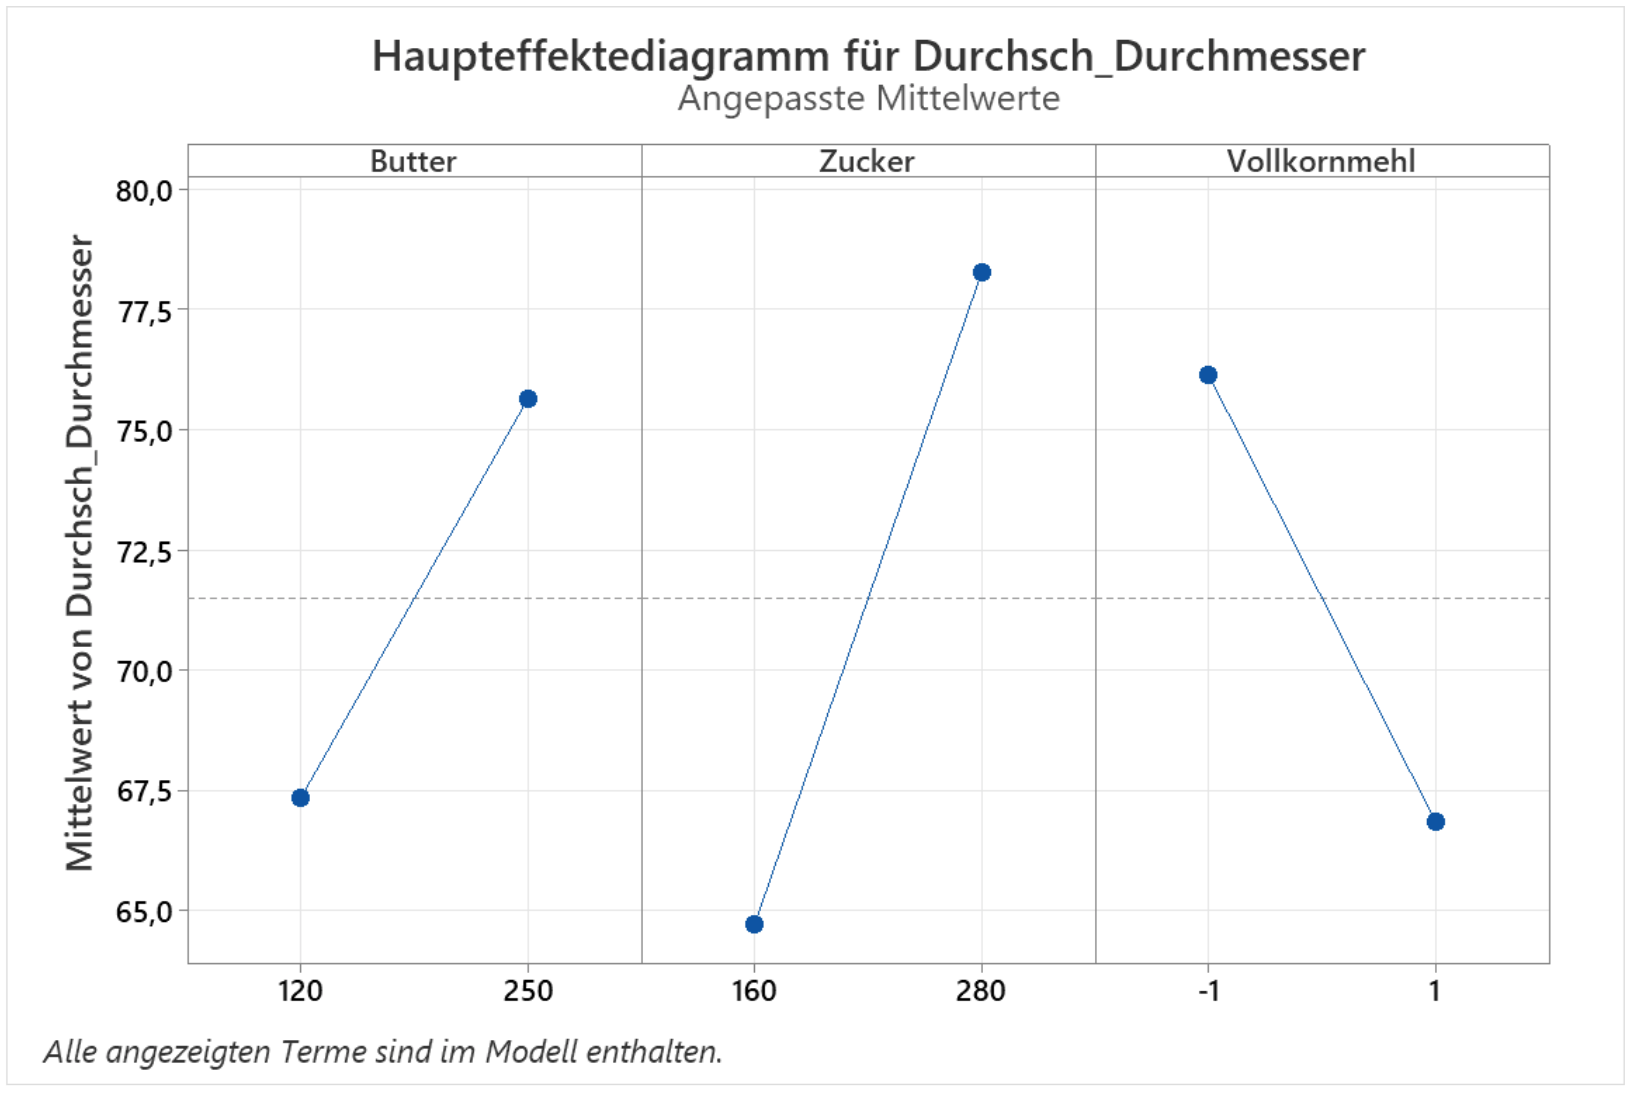
\includegraphics[width=0.7\linewidth]{figures/haupteffekte_diagramm.png}
    \caption{Haupteffekte und deren Wirkung auf den Durchmesser}
    \label{fig:haupteffekte_diagramm}
\end{figure}

Die Regressionsgleichung in kodierter Form für das finale Modell ist wie folgt:

\begin{equation} \label{eq:modell_final}
\begin{split}
\text{Durchsch\_Durchmesser} = & 71,483 - 1,583 \cdot \text{Block\_1} + 0,117 \cdot \text{Block\_2} \\
                               & + 4,146 \cdot \text{Butter} + 6,771 \cdot \text{Zucker} - 4,646 \cdot \text{Vollkornmehl}
\end{split}
\end{equation}